\documentclass{article}
\usepackage{graphicx} % Required for including images
\usepackage{booktabs} % For professional looking tables
\usepackage{amsmath}  % For math symbols if needed
\usepackage{parskip}  % Add space between paragraphs
\setlength{\parindent}{0pt} % Remove paragraph indentation
\usepackage[margin=1in]{geometry} % Set margins to 1 inch

\title{Quantum Eraser Experiment Results: Visibilities and Graphs (2025-05-29)}
\author{Group 13} % Assuming the same group as lab-6-entangled.tex
\date{\today}

\begin{document}
\pagestyle{empty} % No page numbers for a single page doc

% The visibility values V_ON and V_OFF below are placeholders.
% Please replace them with the actual values obtained by running the coincidences.py script.
% The script will print lines like:
% Coincidence Visibility (eraser-on): X.XXX
% Coincidence Visibility (eraser-off): Y.YYY
\begin{table}[h!]
\centering
\begin{tabular}{lcc}
\toprule
\textbf{Condition} & \textbf{Signal LP angle} & \textbf{Visibility (V)} \\
\midrule
Eraser On          & $22.5^\circ$  & 0.481 \\
Eraser Off         & $-22.5^\circ$ & 0.055 \\
\bottomrule
\end{tabular}
\caption{
  Observed visibilities for idler self-interference in the MZI,
  when erasing which-way information from the signal photon (or not)
  in the entangled quantum eraser experiment.}
\end{table}


\begin{figure}[h!]
\centering
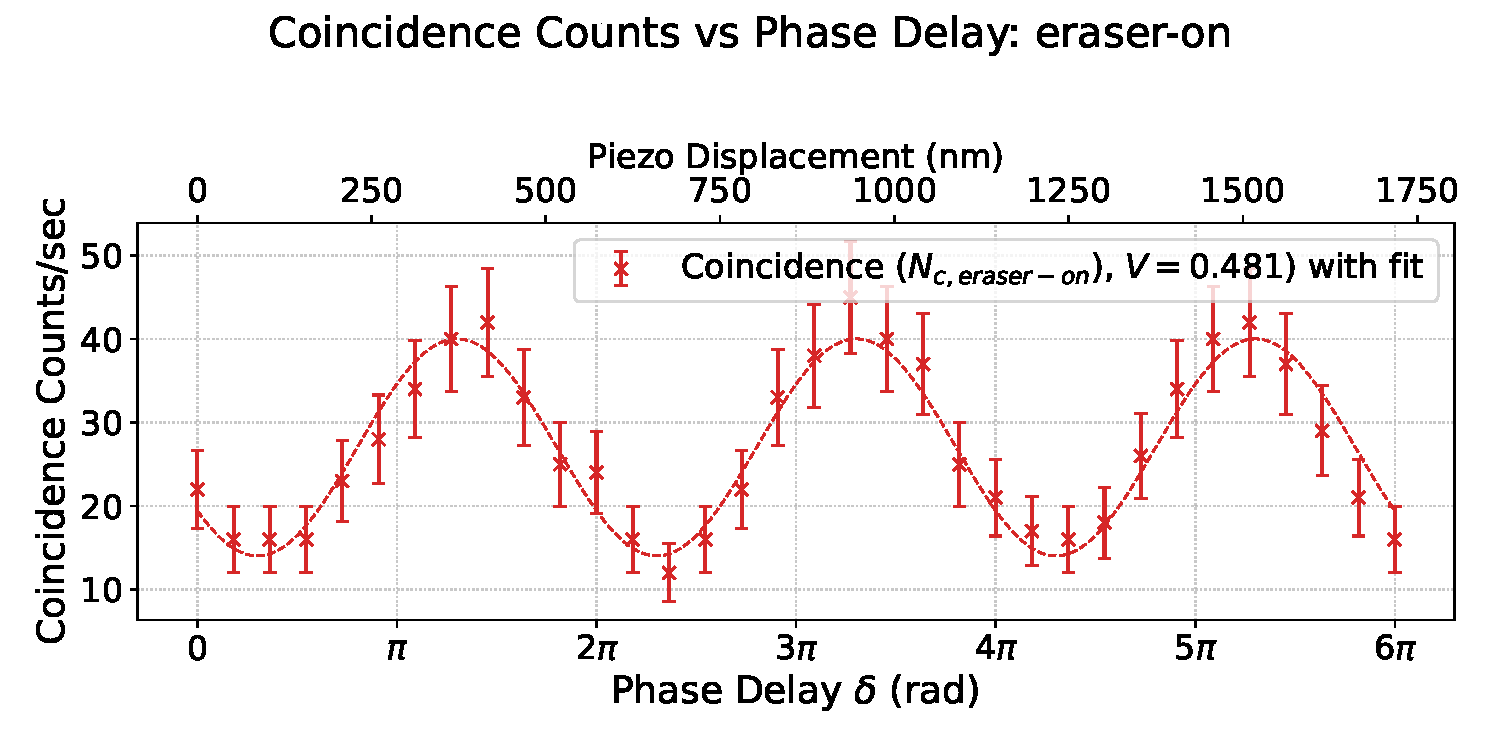
\includegraphics[width=0.6\textwidth]{coincidence_counts_eraser_on.pdf}
\caption{
  Erasing which-way information from the signal photons
  produced high visibility ($V=0.481$) self-interference of the idlers in the MZI.
  Coincidence counts vs Phase Delay with the eraser on.
}
\end{figure}


\begin{figure}[h!]
\centering
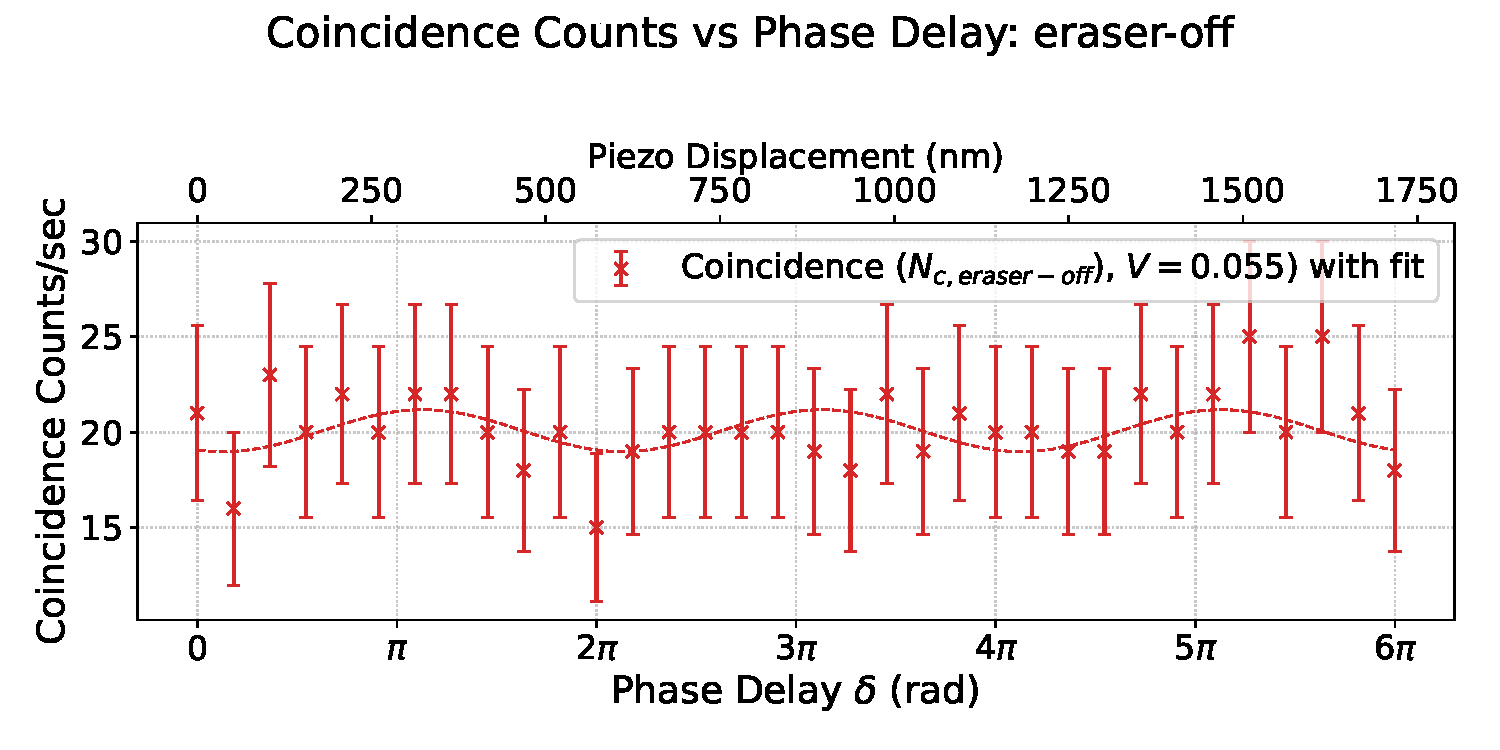
\includegraphics[width=0.6\textwidth]{coincidence_counts_eraser_off.pdf}
\caption{
  Not erasing which-way information from the signal photons
  prevented self-interference of the idlers in the MZI,
  resulting in low visibility ($V=0.055$).
  Coincidence counts vs Phase Delay with the eraser off.
}
\end{figure}

\end{document}
